
\begin{figure}
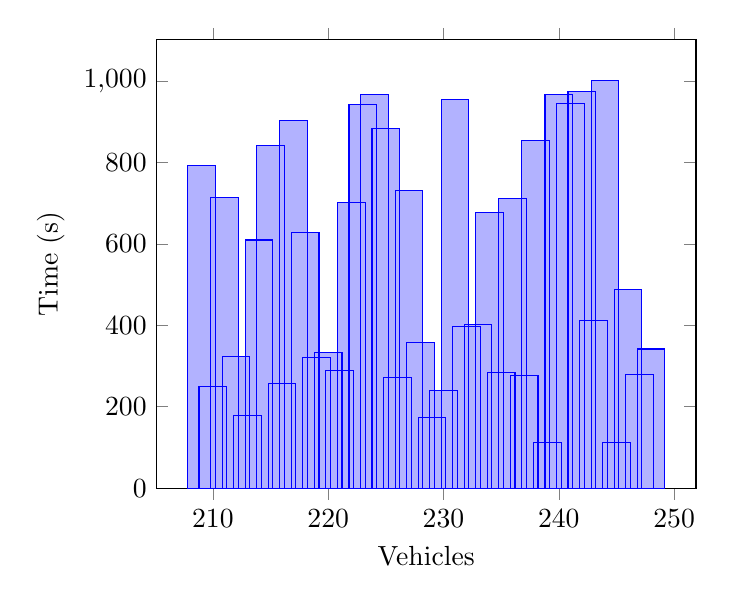
\begin{tikzpicture}
\begin{axis}[
legend style={anchor=west},
xlabel=Vehicles,
ylabel=Time (s),
ymin=0,
ybar,
]
\addplot coordinates {
(230, 241)
(223, 943)
(243, 413)
(210, 250)
(219, 321)
(247, 279)
(232, 397)
(246, 488)
(238, 855)
(221, 289)
(237, 276)
(220, 334)
(242, 975)
(209, 792)
(231, 955)
(224, 968)
(213, 178)
(241, 946)
(234, 677)
(217, 903)
(240, 967)
(239, 112)
(236, 713)
(212, 324)
(233, 402)
(211, 715)
(225, 884)
(218, 629)
(215, 842)
(229, 174)
(214, 610)
(227, 731)
(235, 284)
(222, 703)
(228, 358)
(226, 272)
(216, 257)
(248, 342)
(244, 1002)
(245, 111)
};

\end{axis}
\end{tikzpicture}
\label{tik:time:100:97}
\caption{100 percent diving with GSC on route $97$}
\end{figure}
